% Mingyu Xia (夏明宇, Westlake ID: 20251202247) Homework #i & #j
\documentclass[11pt]{whatsnote}

\usepackage[natbib, style = phys, biblabel = brackets, sorting = none]{biblatex}
\addbibresource{reference.bib}

\coverset{
  title   = Quantum Many-Body Theory,
  author  = \ttfamily \textsc{Mingyu Xia},
  afill   = PhD @Westlake University,
  date    = November 2025,
  extinfo = {\includegraphics[width = .1\paperwidth]{myhsia_seal}},
  head    = string.pdf,
  clogo   = cat.pdf,
  llogos  = {mouse1.png, mouse2.png,
             mouse4.png, mouse5.png}
}

\begin{document}

\maketitle[violet]
\frontmatter
\tableofcontents
\mainmatter

\input{chapter/1_.tex}
% !TeX root = ../main.tex

\chapter{Gaussian Integral}

\section{Free Gaussian Integral}

\[I = \int_{-\infty}^{+\infty} \d x \upe^{-x^2} = \sqrt\pi, ~ I^2 = \pi\]

\subsection{Perturbation expansion of $\mathsf{\int_{-\infty}^{+\infty} \d x \upe^{-x^2-gx^4}}$}

\begin{equation}
  Z(g) = \sum_{n = 0}^\infty \frac{(-g)^n}{n!} \int \d x x^{4n} \upe^{-x^2}
  \label{1.1}
\end{equation}
\begin{equation}
  \int x^{2m}\upe^{-x^2}\d x i
\end{equation}
\emph{Perturbation expansion} is actually divergent: $\lim_{n \to \infty} \ab|\frac{a_{n+1}}{a_n}| \Rightarrow \infty$

The series $Z(g)$ has zero convergence radius.

\section{Feynman Diagram}

\begin{enumerate}
  \item Vertice: $gx^4$
  \begin{tikzpicture}[baseline = (o)]
    \begin{feynhand}
    \vertex (a) at (-1,1);
    \vertex (b) at (1,-1);
    \propag [plain] (a) to (b);
    \vertex (c) at (1,1);
    \vertex (d) at (-1,-1);
    \propag [plain] (c) to (d);
    \vertex [dot] (o) at (0,0) {};
    \end{feynhand}
  \end{tikzpicture}
  \item Propagator: $<x$, $x > = \frac12$
  \begin{enumext}[columns = 2]
    \item $n = 1$:
    \[
      \begin{tikzpicture}[baseline = (o.base)]
        \begin{feynhand}
        \vertex (a) at (-1,1);
        \vertex (b) at (1,-1);
        \propag [plain] (a) to (b);
        \vertex (c) at (1,1);
        \vertex (d) at (-1,-1);
        \propag [plain] (c) to (d);
        \vertex [dot] (o) at (0,0) {};
        \end{feynhand}
      \end{tikzpicture}
      \to
      \begin{tikzpicture}[baseline = (o.base)]
        \begin{feynhand}
          \vertex [grayblob, above] (a) at (0,0) {};
          \vertex [grayblob, below] (b) at (0,0) {};
          \vertex [dot] (o) at (0,0) {};
        \end{feynhand}
      \end{tikzpicture}
      +
      \begin{tikzpicture}[baseline = (o.base)]
        \begin{feynhand}
          \vertex [grayblob, left] (a) at (0,0) {};
          \vertex [grayblob, right] (b) at (0,0) {};
          \vertex [dot] (o) at (0,0) {};
        \end{feynhand}
      \end{tikzpicture}
    \]
    \item $n = 2$:
    \[
      \begin{tikzpicture}[baseline = (o.base)]
        \begin{feynhand}
        \vertex (a) at (-1,1);
        \vertex (b) at (1,-1);
        \propag [plain] (a) to (b);
        \vertex (c) at (1,1);
        \vertex (d) at (-1,-1);
        \propag [plain] (c) to (d);
        \vertex [dot] (o) at (0,0) {};
        \end{feynhand}
      \end{tikzpicture}
      +
      \begin{tikzpicture}[baseline = (o.base)]
        \begin{feynhand}
        \vertex (a) at (-1,1);
        \vertex (b) at (1,-1);
        \propag [plain] (a) to (b);
        \vertex (c) at (1,1);
        \vertex (d) at (-1,-1);
        \propag [plain] (c) to (d);
        \vertex [dot] (o) at (0,0) {};
        \end{feynhand}
      \end{tikzpicture}
      \to
    \]
  \end{enumext}
\end{enumerate}
Symmetry factor.

\section{Finite $n$ still good for $g$-expansion}
\begin{equation}
  Z_\text{exact}(g) = \frac12\sqrt{\frac\pi g} \upe^{1/(8g)} K_{1/4}\ab(\frac{1}{8g})
\end{equation}
$K_{1/4}$ is modified Bessel function.

\begin{tikzpicture}
  \draw [->] (-.5,0) -- (3,0) node [below] {$N$};
  \draw [->] (0,-.5) -- (0,3) node [left, align = right] {error\\$Z_n(g)$ -- $Z_\text{exact}(g)$};
  \draw [dashed, rounded corners] (0,2.5) -- (1.5,.5) -- (3,2.5);
\end{tikzpicture}

Around $N = 13$: it starts going out.

Kondo Problem: to 1 or 2 order.

\noindent\rule{\linewidth}{1pt}

From \eqref{1.1}, we have
\begin{align}
  Z(g)  & = \frac1{g^{1/4}} \int \d y e^{-y^4-y^2/g^{1/2}}\\
        & = \frac1{g^{1/4}} \sum_{m = 0}^\infty \frac{(-1)^m}{m!} \frac{1}{g^{m/2}} \underset{\frac12\frac{\Gamma\left(\frac m2 + \frac14\right)}{g^{m/2} + 1/4}}{\underbrace{\int \d y y^{2m} e^{-y^4}}} \text{(Taylor Expansion)}\\
  \ab|\frac{a_{m+1}}{a_m}| & \to \frac{1}{\sqrt{2g}} \cdot \frac1{\sqrt m} \to 0
\end{align}
Then, $Z(1/g)$ cmverges $(0,+\infty)$

Large $y$, no matter how small $g$ is, $y^4$ term dominates.

\section{Multi-variable Gaussian Integral}

Just means we have found
\begin{equation}
  \int \d x_1 \d x_2 \ldots\d x_N \upe^{-[x][M][x]} =
  \frac12\int \d y_1 \cdots\d y_N \upe^{-[y]u^\dagger Mu[y]}
\end{equation}
\begin{enumext}[columns = 2]
  \item $[x] = (x_1,\ldots,x_N)$
  \item $[M] = (M_{ij})$.
\end{enumext}

Diagonalise $M$: $[x] \to u[y]$, $M \to \pdiagmat[empty = {}]{\ddots, \ddots, \ddots}$,
$u^\dagger Mu = \pdiagmat[empty = {}]{\ddots,\ddots,\ddots}$.

\begin{framed}
  Add interaction:
  \begin{equation}
    \int \d x_1 \ldots \d x_N \upe^{-\sum_{i = 1}^N x_i^4 g}
  \end{equation}
\end{framed}

Consider strong coupling expansion:
\begin{equation}
  \int \d x_1 \cdots \d x_n \upe^{-\sum x_{i1}, x_{i2}, \ldots, x_{in} g_{12}^{34}}
\end{equation}
\begin{equation}
  \int \d y_1 \cdots \d y_N = \upe^{-y^4}
\end{equation}
\input{chapter/3_.tex}
\input{chapter/4_.tex}
\input{chapter/5_.tex}
% !TeX root = ../main.tex

\chapter{More Green's Functions}

\section{Green's function}

\subsection{GFs differential Eqs}

\begin{equation}
  \odv*[2]fx + S(x) f(x) = 0, \qq{or} \hat{\mathcal L} f = 0
\end{equation}
then we can construct $\odv*[2]gx = S(x)$, $f = \int \d x g \cdot S(x)$.

\subsection{GF as propagators in Q.M.}

From the S.E.
\[
  \iu \hbar \pdif t\psi = H\psi
\]
we get the G.F. $G = \braket<x|U|x'>$. To be specific
\begin{equation}
  \ab(\iu\hbar \pdif t + \frac{\hbar^2}{2m}\nabla^2) G_{t,x;t',x'} = \delta(t - t') \delta(x - x')
\end{equation}
which is the EOM, and $G_{t,x;t',x'}$ is the P.I.

\subsection{One particle GF \&  real frequency/real time}

Consider the indicate label $\lambda$, the GF
\begin{equation}
  G_{\lambda\lambda'}
= -\iu \braket<\phi|\mathcal T\psi_\lambda(t) \psi_{\lambda'}^\dagger(t')|\phi>
\end{equation}
where
\begin{equation}
  \mathcal T \hat\psi_\lambda(t) \hat\psi_{\lambda'}^\dagger =
  \begin{cases}
    \psi_\lambda(t) \psi(t'), & t > t'\\
    \pm \psi_\lambda^\dagger(t') \psi_\lambda(t), & t < t'
  \end{cases}
\end{equation}
and the Bosons for $+$ and Fermions for $-$. To combine,
\begin{equation}
  \mathcal T \hat\psi_\lambda(t) \hat\psi_{\lambda'}^\dagger
= \theta(t - t') \psi_\lambda(t) \psi_{\lambda'}^\dagger(t') \pm \theta(t' - t) \psi_{\lambda'}^\dagger(t') \psi_\lambda(t)
\end{equation}
when we take the time derivative,
\begin{equation}
  \begin{aligned}
  \iu\pdif t G & = \delta(t - t') (\psi_\lambda \psi_{\lambda'}^\dagger \mp \psi_{\lambda'}^\dagger \psi_\lambda) + \braket<\mathcal T[\psi, \iu t], \psi_{\lambda'}>\\
  & =
  \begin{cases*}
    \delta(t - t') [\psi_\lambda, \psi_{\lambda'}^\dagger] = \delta(t - t') \delta_{\lambda\lambda'}, & Bosons\\
    \delta(t - t') \{\psi_\lambda, \psi_{\lambda'}^\dagger\} = \delta(t - t') \delta_{\lambda\lambda'}, & Fermions
  \end{cases*} +  \braket<\mathcal T[\psi, \iu t], \psi_{\lambda'}>
  \end{aligned}
\end{equation}
Classically, the commutator is the Poisson bracket $\{\quad\} = \delta_{ij}$.
For bosons and fermions, $\delta_{\lambda\lambda'}$ are all canonical operators,
also exist for many-body operators.

\subsection{Linear response problem: double time -- GFs for arbitrary operators}

\begin{gather}
  G_{\hat A,\hat B}^\text{ret}
= -\iu\theta(t - t') \ab<\braket<[\hat A(t), \hat B(t')]_\pm>>\\
  G_{\hat A,\hat B}^\text{adv}
= +\iu\theta(t' - t) \ab<\braket<[\hat A(t), \hat B(t')]_\pm>>
  G_{\hat A,\hat B}^\text{C} = -\iu\ab<\braket<\mathcal T_\pm(\hat A(t) \hat B(t'))>>
\end{gather}
where $\text C = \text{Causal} = \text{$T$-ordered}$, and
\[
  \ab*<\braket<\hat A(t), \hat B(t')>> = \braket<\Phi|(\hat A(t) - \ab<\hat A(t')>) (\hat B(t') - \ab<\hat B(t')>)|\Phi> = \Tr[\rho \cdots]
\]
and $\braket<A> = \braket<\Phi|A|\Phi>$, also for $B$.

\subsection{Spectral Density of GFs}

\begin{equation}
  S_{AB}(t,t') = \frac1{2\pi}\braket<[A(t), B(t')]_\xi>
\end{equation}
If set $t \to t'$, $G[0] = S_{AB}(t = t')$,
and we can prove the quantities should evolve to
\[
  \braket<A(t)B(t')> = \braket<A(t-t')B(0)>
\]

\subsection{Spectral representation of GF}

\begin{equation}
  H\ket|E_n> = E_n \ket|E_n>,~
  \sum_n \ketbra|E_n><E_n| = \mathbbm 1,~
  \braket<E_n|E_m> = \delta_{nm}
\end{equation}
Take the trace with the exact eigenstates
\begin{equation}
  \begin{aligned}
    \Tr[\upe^{-\beta H} A(t) B(t')] &
  = \sum_{nm} \braket<E_n|\upe^{-\beta H} A(t)|E_n>\braket<E_m|B(t')|E_n>\\
& = \sum \upe^{-\beta E_n} \braket<E_n|A^{(t')}|E_m>\braket<E_m|B^{(t')}|E_m>\\
& = \sum \upe^{-\beta E_n} \upe^{\frac\iu\hbar (E_n-E_m)(t-t')}
    \braket<E_n|\hat A|E_m>\braket<E_m|\hat B|E_n>
  \end{aligned}
\end{equation}
Then we can have
\begin{equation}
  S_{AB}[E] = \sum_{n,m} \delta(E - (E_n - E_m)) (\upe^{\beta E} - \epsilon)
  \braket<E_n|B|E_m>\braket<E_m|A|E_n> \upe^{-\beta E_n}
\end{equation}
For the fourier transformation of the step function
\begin{align*}
  \theta(t - t') & = \frac\iu{2\pi} \int_{-\infty}^{+\infty}
  \d E \frac{\upe^{-\iu E(t-t')}}{E + \iu 0^+},\\
  \theta(t' - t) & = \frac\iu{2\pi} \int_{-\infty}^{+\infty}
  \d E \frac{\upe^{-\iu E(t-t')}}{E + \iu 0^-}
\end{align*}
Then
\begin{gather}
  G[E] = \frac{f_e(E\cdots)}{f_2(E\cdots)} = \frac{f_1(E)}{\prod(E - E_i)} = \sum_i \frac{g_i(E)}{E - E_i + \iu\sgn[E_i]}\\
  f_2(E\cdots) = \sum_n (E^na_n + E^{n-1}a_n \cdots) = \sum_{i=1}^n(E - E_i)
\end{gather}
Then, the Hilbert transformation of the retard/advanced/canonical GF and $S$-matrix can be written as
\begin{align}
  G^\text{ret}(E) & = \int_{-\infty}^{\infty} \d E' \frac{S_{AB}(E')}{E - E' + \iu 0^+},\\
  G^\text{adv}(E) & = \int_{-\infty}^{\infty} \d E' \frac{S_{AB}(E')}{E - E' + \iu 0^-},\\
  G^\text{C}(E) & = \int_{-\infty}^{\infty} \d E' \frac{S_{AB}(E')}{E - E' + \iu\sgn[E'] 0^+},\\
  S_{AB}(E) & = \frac\iu{2\pi} [G_{AB}(E + \iu 0^+) - G_{AB}(E - \iu 0^+)]
= -\frac1\pi \Im[G_{AB}^\text{ret}(E)].
\end{align}

\section{GFs continent}

For arbitrary operator $A$ and $B$, which could be both Fermionic or Boson
\begin{equation}
  \iu G_{AB}^c = -\iu\ab[\theta(t - t') \braket<A(t) B(t')> \pm
    \theta(t' - t) \braket<B(t')A(t)>]
\end{equation}
where $\braket<A(t)B(t')>$ and $\braket<B(t')A(t)>$ is so-called the greater and lesser Green functions: $G^>$, $G^<$, and $[c,c^\dagger]_\xi = 1$.
The retarded/advanced Green function are defined as
\begin{align}
  G_{AB}^\text{ret} & = -\iu\theta(t - t') \braket<[A(t), B(t')]_\xi>\\
  G_{AB}^\text{adv} & = +\iu\theta(t' - t) \braket<[A(t), B(t')]_{-\xi}>
\end{align}
Now the solution will like
\[
  \frac{1}{E - E_i + \iu\sgn(E)}
\]
where $\sgn(E)$ can be $0^+$ (retarded Green function) and $0^-$ (advanced green functioin). The Heaviside function satisfies the Fourier Transformation
\[
  \theta(t - t') = \frac1{2\pi} \int \d x \frac{\upe^{\iu x(t-t')}}{x + \iu 0^+}
\]
If the state $\Phi_0$ is applied to $G^<$, i.e.,
\[
  \braket<\Phi_0|B(t')A(t)|\Phi_0> \to \Tr[\rho A(t)B(t')]
\]
where
\[
  G[t,t'] = G(t - t', 0) = G(0, t - t')
\]
We define
\begin{equation}
  S_{AB}(E) = \braket<A(t)B(t')>
\end{equation}
Then the retarded Green function becomes
\begin{equation}
  G_{AB}^\text{ret}(E) = \int \d E' \frac{S_{AB}(E)}{E - E' + i0^+} \sim \delta(E - E')
\end{equation}
and we can get $S_{AB}(E)$ from the Green function
\begin{equation}
  S_{AB}(E) = \mp\frac1\pi \Im G^\text{ret/adv}
\end{equation}
and $-\frac1\pi \Im(G[c_k, c_k^\dagger]) = A_k(\omega)$.
Typically,
\begin{align}
  S_{AB}(t,t') & = \braket<A(t)B(t')>,\\
  S_{BA}(t,t') & = \braket<B(t')A(t)>,
\end{align}
If one is measuring $k > k_F$, then $\braket<c_k^\dagger, c_k> = 0$,
$\braket<c_k, c_k^\dagger> = 1$; $k < k_F$.
$\braket<S^+(t)S^-(t')>$,
$\braket<S^-(t')S^+(t)>$.

\subsection{Spectral density}

The commutator and anticommutator
\begin{align*}
  S_{AB}^{(-)} & = \braket<\{A(t), B(t')\}>,\\
  S_{AB}^{(+)} & = \braket<[A(t), B(t')]>,
\end{align*}
If we define $\tilde A = A - \braket<A>$, $\tilde B = B - \braket<B>$,
then $S_{AB}^{(+)} = S_{\tilde A\tilde B}^{(+)}$,
\begin{equation}
  S_{AB}^{(\epsilon)}(E) = S_{\tilde A\tilde B}^{(\epsilon)}(E) + (1 - \epsilon) DS(E)
\end{equation}
which is so-called spectral theorem.

Expand the $\tilde A$, $\tilde B$ term
\[
  \braket<\{(A - \braket<A>)(B - \braket<B>)\}> = \braket<\{A,B\}> - 2\braket<A>\braket<B> + \braket<A>\braket<B>
\]
where we can define
\begin{equation}
  D = -2\braket<A>\braket<B> = \frac1Z \sum_{n,m}^{E_n=E_m}\upe^{-\beta E_n}
  \braket<E_n|B|E_m>\braket<E_m|A|E_n>
\end{equation}
We can get the relation between $S$
\[
  S[A,B] = \frac12(S^{(-)} + S^{(+)}), \quad
  S[B,A] = \frac12(S^{(-)}  S^{(+)})
\]
If taking the limit
\[
  \lim_{E\to0}EG^(\epsilon)(E) = (1 - \epsilon) D
\]
Keldysh-formula.

From the EOM of $\tilde G^\pm$
\begin{gather}
  \iu\pdif t \tilde G^{+,c} = \delta(t) \braket<[A,B]> + \Gamma^+ (ee)= \delta(t) \tilde G^{(-)}(t = 0) + \Gamma^+\\
  \iu\pdif t G_{AB}^{-,c} = \delta(t) \braket<\{A,B\}> + \Gamma^-
\end{gather}
The COBS are $\{\hat u^\alpha\}$, where$u^\alpha u^\beta = f^{\alpha\beta}_\gamma u^\gamma$. The commutator
\[
  \braket<[u^\alpha, u^\beta] = a^{\alpha\beta},
  \braket<\{u^\alpha, u^\beta\}> = c^{\alpha\beta}_\gamma u^\gamma>
\]
Since $[\braket<S^+, S^z>] = \braket<S^x>$.

\section{Finite-$T$ Green function \& Matsubara method}

Denote $\braket<\quad>_\text{thermal}$, then acting
\begin{equation}
  \mathcal T \upe^{\iu \int \d t H} \xleftrightarrow{t\leftrightarrow\iu\tau}
  \upe^{-\int_0^\beta H\tau \d\tau}
\end{equation}

Starting from the thermal average
\begin{equation}
  \braket<A(t)B(t')> = \braket<A(t - t')B(0)>
\end{equation}
considering setting $t \to t - \iu\beta$
\[
  Z \tr[\upe^{-\beta H} \upe^{\iu Ht} A \upe^{-\iu Ht} \upe^{+\iu Ht'}B\upe^{-\iu Ht'}]
\]
The trace $\Tr[AB\cdots C]$ is invariant under cyclE. The thermal average
\begin{equation}
     \braket<A(t-\iu\beta)B(t')>_\text{thermal}
  = \Tr[\upe^{-\beta H} \upe^{\iu H(t-\iu\beta)A\upe^{-\iu(i)}}]
  = \Tr[B(t') \upe^{\iu Ht} A \upe^{-\iu Ht} \upe^{-\beta H}]
  = \Tr[\upe^{-\beta H} B(t') A(t)]
\end{equation}
Som we fund that when $t = t' = 0$
\[
  \braket<A(\tau=\beta)B(0)>_\beta = \braket<A(\iu\tau)B(0)>
\]
and we obtain the EOM and solution
\[
  -\pdv*{A(\tau)}\tau = [A(\tau), H], \quad A(\tau) = \upe^{H\tau} A(0) \upe^{-HE}
\]
Sincee
\[
  \theta(\tau) = \begin{cases*}
    1, & if $\tau > 0$\\
    0, & if $\tau < 0$
  \end{cases*}
\]
Then $T_\tau\{A(\tau) B(\tau')\}$.
\[
  \braket<A(t;)B(t')> \Rightarrow \tau,
  G_{AB}^M (\tau,\tau') = -\braket<\mathcal T_\tau(A(\tau, B(\tau')))> = G_{AB}^M (\tau-\tau',0)
\]
\[
  G_{AB}^M (\tau-\tau',0) = \epsilon G_{AB}^M(\tau - \tau' + n\beta, 0)
\]
To proof that,
\begin{proof}
  \begin{equation}
    G_{AB}^M (\tau-\tau',0) = \mathcal EG_{AB}^M(\tau-\tau' + n\beta,0)
  \end{equation}
  then
  \begin{align*}
    G_{AB}^M (\tau-\tau' + \beta,0) &
  = \Tr[\upe^{-\beta H} \upe^{H(\tau-\tau'+\beta)A}
        \upe^{-H(\tau-\tau'+\beta) B}]\\
  & = \Tr[\upe^{-\beta H} B \upe^{H(\tau-\tau') A \upe^{-H(\tau-\tau')}}]
  = G_{AB}^M [B(0) A(\tau-\tau')] = \epsilon G_{AB}^M (\tau-\tau',0)
  \end{align*}
  For boson: periodic; for fermion: antiperiodic.
  Then apply the Fourier transformathon, we have Matsubara freq.
  Then let $E \to \iu E_n$, $E_n = 2m\pi/\beta$, or $E_n = (2n + 1)\pi/\beta$,
  where $\tau\in(-\beta,\beta)$.
  \[
    \int \d\omega \upe^{\iu\omega t} G[\omega] \ldots \Rightarrow
    \sum_{n=-\infty}^{+\infty} \upe^{\iu E_n\tau} G[\iu E_n] (\ldots)
    \Rightarrow \sum_{n=-\infty}^{+\infty} \upe^{\iu E_n\tau} G[E_n]
  \]
  then
  \begin{equation}
    G[E_n] = \int \d E' \frac{S_{AB}(E')}{\iu E_n - E' + \iu0^+}
  \end{equation}
  along the contour
  \[
    \sum_{n=-\infty}^{+\infty} f(\iu E_n) = \oint \d z \frac{1}{\upe^{\beta z}\mp 1} f(z)
  \]
  to calculate the residue, let $\upe^{\beta z = \pm 1}$, then $\tau\to\beta$, we have
  \begin{equation}
    \sum_n \upe^{\iu E_nt} G[\iu E_n]
  = \int \d z \d z' \frac{\upe^{\tau z} S_{AB}(E')}{(\upe^{\beta z} \pm 1) (z - E')}
  = \int \d z \d z' f^\text{BF}(z) \frac{S_{AB}(E')}{(z - E')}\bigg|_{\tau\to\beta}
  \end{equation}
  SPEOM: $G$.
\end{proof}

\section{Examples of GFs}

\begin{example}
  For fermions, the Hamiltonian
  \[
    H = H_0 - \mu N = \sum \epsilon_k c_k^\dagger c_{k\sigma}
  \]
  So the free fermion
  \[
    \ket|\Phi> = \prod_{k<k_F, \epsilon_k < 0} c_{k\sigma}^\dagger \ket|0>
  \]
  then
  \[
  \]
  where $n_k = \theta(k_F - k]$. THen
  \[
    \braket<\Phi|c_{k\sigma}(t) c_{k'\sigma'}^\dagger(t')|\Phi> = \delta_{\sigma\sigma'} \delta_{kk'} \upe^{-\iu\epsilon_k} \braket<\phi|c_{k\sigma}c_{k\sigma}^\dagger|\phi>
    = \delta_{\sigma\sigma'} \delta_{kk'} \upe^{-\iu\epsilon_k(\tau-\tau')} (1 - n_k)
  \]
  So, the Green function
  \[
    G^c(k,t) = -\iu\ab[(1 - n_k)\theta(t) - n_k\theta(-t)]\upe^{-\iu\epsilon_kt}
  = \begin{cases*}
    -\iu\theta(|k| - k_F)\upe^{-\iu\epsilon_k t}, & $t > 0:$ particle\\
    \iu\theta(k_F - |k|)\upe^{-\iu\epsilon_k t}, & $t < 0:$ holes\\
  \end{cases*}
  \]
  From the Fourier transformathon
  \[
    G^c(k,\omega) = -\iu\ab(\frac{\theta(k_1 - k_F)}{\delta-\iu(\omega - \epsilon_k)} - \frac{\theta(k_1 - |k|)}{\delta+\iu(\omega - \epsilon_k)})
    \to
    \frac1{\omega - \epsilon_k + \iu\delta^+\sgn(|k| - k_F)}
  \]
  where $\theta(k_1 - k_F) \sim 1 - n_k$, $\theta(k_f - |k|) \to n$. i.e., the valid for any eigenstate of H
  \begin{equation}
    \iu\pdif t G = \delta(t) + \epsilon G
  \end{equation}
  Then,
  \[
    G^c = \frac1{\omega - \epsilon_k + \iu\delta^+\sgn(\epsilon_k)}
  \]
  $\prod_{k\in(k_1,k_0)} c_k^\dagger\ket|0>$
  \[
    \frac{1-n_k}{\omega - \epsilon_k} + \frac{n_k}{\omega - \epsilon_k} \Rightarrow\frac{1}{\omega - \epsilon_k}
  \]
  From this, we have
  \[
    E = \sum_k \epsilon_k \braket<n_k> \sim \int G \epsilon \d k
  \]
  and then, we can minimize the energy: $\delta E = 0$,
  for $S_{AB}$ and $S_{BA}$.
\end{example}

\begin{example}[Free boson capped]
  \textbf{No BEC}
  The Hamiltonian
  \[
    H = \sum \omega_q b_q^\dagger b_q
  \]
  and the Green functions
  \[
    G[b_q, b_q^\dagger](k,\omega) = \frac{1}{\omega - \omega_q}
  \]
  $G[\phi_q, \Phi_q]$, where $\Phi_q = b_q + b_q^\dagger$.
  \[
    H_0 = \sum_k \epsilon_k b_k^\dagger b_k
  \]
  \textbf{BEC}
  The ground state is
  \[
    \ket|\Psi> = (a_0^\dagger)^N \ket|0>
  \]
  that is called the BEC.
  when $\epsilon_k \to 0$, $N/V = n_0\big|_{L\to\infty, N\to\infty}$.
  The Green function
  \[
    G_0(k,\omega) = G(a_{k:\epsilon_k = 0}, a_k^\dagger) (k,\omega)
  = \underbrace{-\iu(2\pi)^d n_0 \delta(k) \delta(\omega)}_\text{Coherent Part} + \underbrace{\frac1{\omega - \epsilon_k + \iu0^-}}_\text{Incoherent Part}
  \]
  The interaction Hamiltonian
  \[
    H_\text{int} = g\sum_{k,k'} a_k^\dagger a_{-k}^\dagger a_{k'} a_{-k'}
  \]
  When acting on $\ket|\Psi>$, $k' = 0$
  \[
    H_\text{int} \ket|\Psi> \sim
    H_\text{eff, int} = \sum_{k\neq0} g n_0 \ab(a_k^\dagger a_k + \frac12 a_k^\dagger a_{-k}^\dagger + \frac12a_{-k}a_k), \quad
    H_{B,E} = \sum_{k\neq0} \epsilon_k a_k^\dagger a_k
  \]
  When acting on $\bra<\Psi|>$, $k = 0$
  \[
    \bra<\Psi|H_\text{int}
  \]
  then $a_0\ket|\psi_0> \sim \sqrt{n_0}\ket|\Psi_0>$
  In total, $H_B = H_\text{eff, int} + H_{B, E}$.
  Since Bogolinbov transformation
  \[  
  b_k = u_ka_k - v_ka_{-k}^\dagger
  \]
  Then
  \[
    E_k = \sqrt{\epsilon_k(c\epsilon_k + 2gn_0)} \approxeq \sqrt{\frac{k^2}{2\pi}\ab(\frac{k^2}{2\pi} + 2gn_0)} \approxeq |k| \sqrt{gn_0}/m
  \]
  which is so-called Goldstone mode.
  The Green function
  \[
    \iu \pdif t G = \delta + \epsilon_{k_0}G + \braket<[a_{k_{0'}, H_\text{inf}}], a_{k'}^\dagger> \to
    \braket<g\sum_{k,k'} a_k^\dagger a_k a_k \delta_{k,k'}> ...
  \]
  ...
  Bascially we have $H_0 \ket|\psi_0>$,
  by adding $\delta H$, we have
  \[
    G_0 + \delta G \propto \delta H / \propto H_0 \delta\psi
  \]
\end{example}

\section{Free spin wave / magnos}

* Most accurate to know the Hamiltonian of magnetic field: Applied a strong field
  \[
    H_0 = -B \sum_j S_j^z
  \]
  The ground state
  \[
    \ket|\Psi> = \ket|\uparrow\uparrow \cdots>
  \]
  Then
  \[
    \delta H = \sum T_{ij}^+ (S_i^+ S_j^- + S_i^- S_j^+) + \sum J_{ij}^z S_i^z S_j^z
  \]
  Since $[S_i^+, S_j^-] = \delta_{ij} 2\braket<S_i^z>$, $\{S_i^+, S_i^- = 1\}$, $\{S_i^+, S_j^-\} \neq 0$, $[S_i^+, S_i^z] = S_i^+$
  The correlation function
  \begin{multline*}
    \iu \pdif x [S^+, S_{-j}^-] = \delta_{ij}2\braket<S_i^z> \delta(t) + \braket<\underbrace{[S^+, H_0]}_{B\braket<S_i^+, S_f^->}, S_f^->
    + \braket<[S^+, \delta H^+], S^->\\
    + J^2 \braket<S_j^z> \braket<S_i^+, S_f^->
    + J^z \braket<S_i^z> \braket<S_j^+, S_f^->
    + \braket<[S^+, \delta H^+], S^->
    + J_{ij}^+ \braket<2S_i^z; S_j^+; S_f^->
  \end{multline*}
  Then do the Foruier Transform
  \[
    \omega G[S_i^+, S_f^-] \approxeq 2\braket<S^z> + B\braket<S_i^+, S_f^-> + \sum_{\braket<ij>} J_{ij} 2\braket<S_i^z> \braket<S_j^+, S_f^->
  \]
  Acting $\pdif t$, summing over possible spin moments.
  Finally, this can be
  \[
    \omega G[S^+, S^-](k, \omega) = 2\braket<S^z> + BG + 2\braket<S^z> J\tilde \epsilon_k
  \]
  \[
    G \approxeq \frac{2\braket<S^z>}{\omega - B - 2J^+ \epsilon_k}
  \]
  Another:
  \[
    H_0 = \sum_{\braket<ij>}J_{ij}^z S_i^z S_j^z, \quad
    \delta H = \sum J_{ij}^+ (S_i^+ S_j^- + \text{H.c.})
  \]
  If $J^z < 0$, then FM; If $^z > 0$: then AFM.
  \[
    \ket*|\substack{\uparrow \uparrow\\\uparrow \uparrow}>, \quad
    \ket*|\substack{\uparrow \downarrow\\\downarrow \uparrow}>
  \]
  are all the classic type: SSB.
  \begin{framed}
    For Ruanfum SSB
    \[
      H = \sum J \bm S \cdot \bm S, \quad [\rho, H] \neq 0
    \]
  \end{framed}
  \[
    \omega G = 2\braket<S^z> + \sum_{\braket<ij>} J_{ij}^z \braket<S_j^z> G[S_i^+, S_f^-]
  + \sum_{\braket<ij>} J_{ij}^z \braket<S_i^z> G[S_j^+, S_f^-]
  + \sum J^+ 2\braket<S_i^z> G[S_j^+, S_f^-]
  \]
  For FM:
  \[
    \omega G = 2\braket<S^z> + 4J^z \braket<S^z> G + \braket<S^z> J^z \epsilon_k G + \braket<S^z> J^2 \epsilon_k G
  \]
  then
  \[
    \omega G = 2\braket<S^z> + (4J^z \braket<S^z> + (\braket<S^z> J^z + \braket<S^z> J^z)\epsilon_k)F
  \]
  then the Green function is
  \[
    G = \frac{2\braket<S^z>}{\omega - 4J^+ \braket<S^z>} + \epsilon_k J^z (1 + J^z/J^+)
  \]
  so-called renormalization of (effective) mass of magon.

For the anti-ferron $\ket*|\substack{\uparrow \downarrow\\\downarrow \uparrow}>$
\[
  \begin{pmatrix}
    G[S_A^+ S_A^-] & G[S_B^+ S_A^-]\\
    G[S_A^+ S_B^-] & G[S_B^+ S_B^-]
  \end{pmatrix}
\]
Assume $k - k' = nQ$, $Q = (\pi, \pi)$.
\[
  \begin{pmatrix}
    G[k,k] & G{k+Q,k}\\
    G[k,k+Q] & G[k+Q,k+Q]
  \end{pmatrix}
\]
\[
  \omega [G] =
  \begin{pmatrix}
    2\braket<S^z>_A &\\
    & 2\braket<S^z>_B
  \end{pmatrix} +
  \begin{pmatrix}
    J^z\epsilon_k & J^z\epsilon_k\\
    -J^z\epsilon_k & -J^z\epsilon_k
  \end{pmatrix}
\]
where $\epsilon_{k+Q} = -\epsilon_k$.
Eventually we will find that
\[
  \sqrt{\epsilon_k(\epsilon_k + J^z)} \propto k
\]
AFM: Spin-wave.
In the $k$-space, the $\cos k$ will flipped.
For FM: $\epsilon_k \propto k^2$.

Only consider the very simple ground state
$\ket|\Psi>_0$.

$G_{kk} \sim G_{AA}$, $k \in \text{First Brillouin Zone}$
\begin{center}
  \begin{minipage}{.48\linewidth}
    \centering
    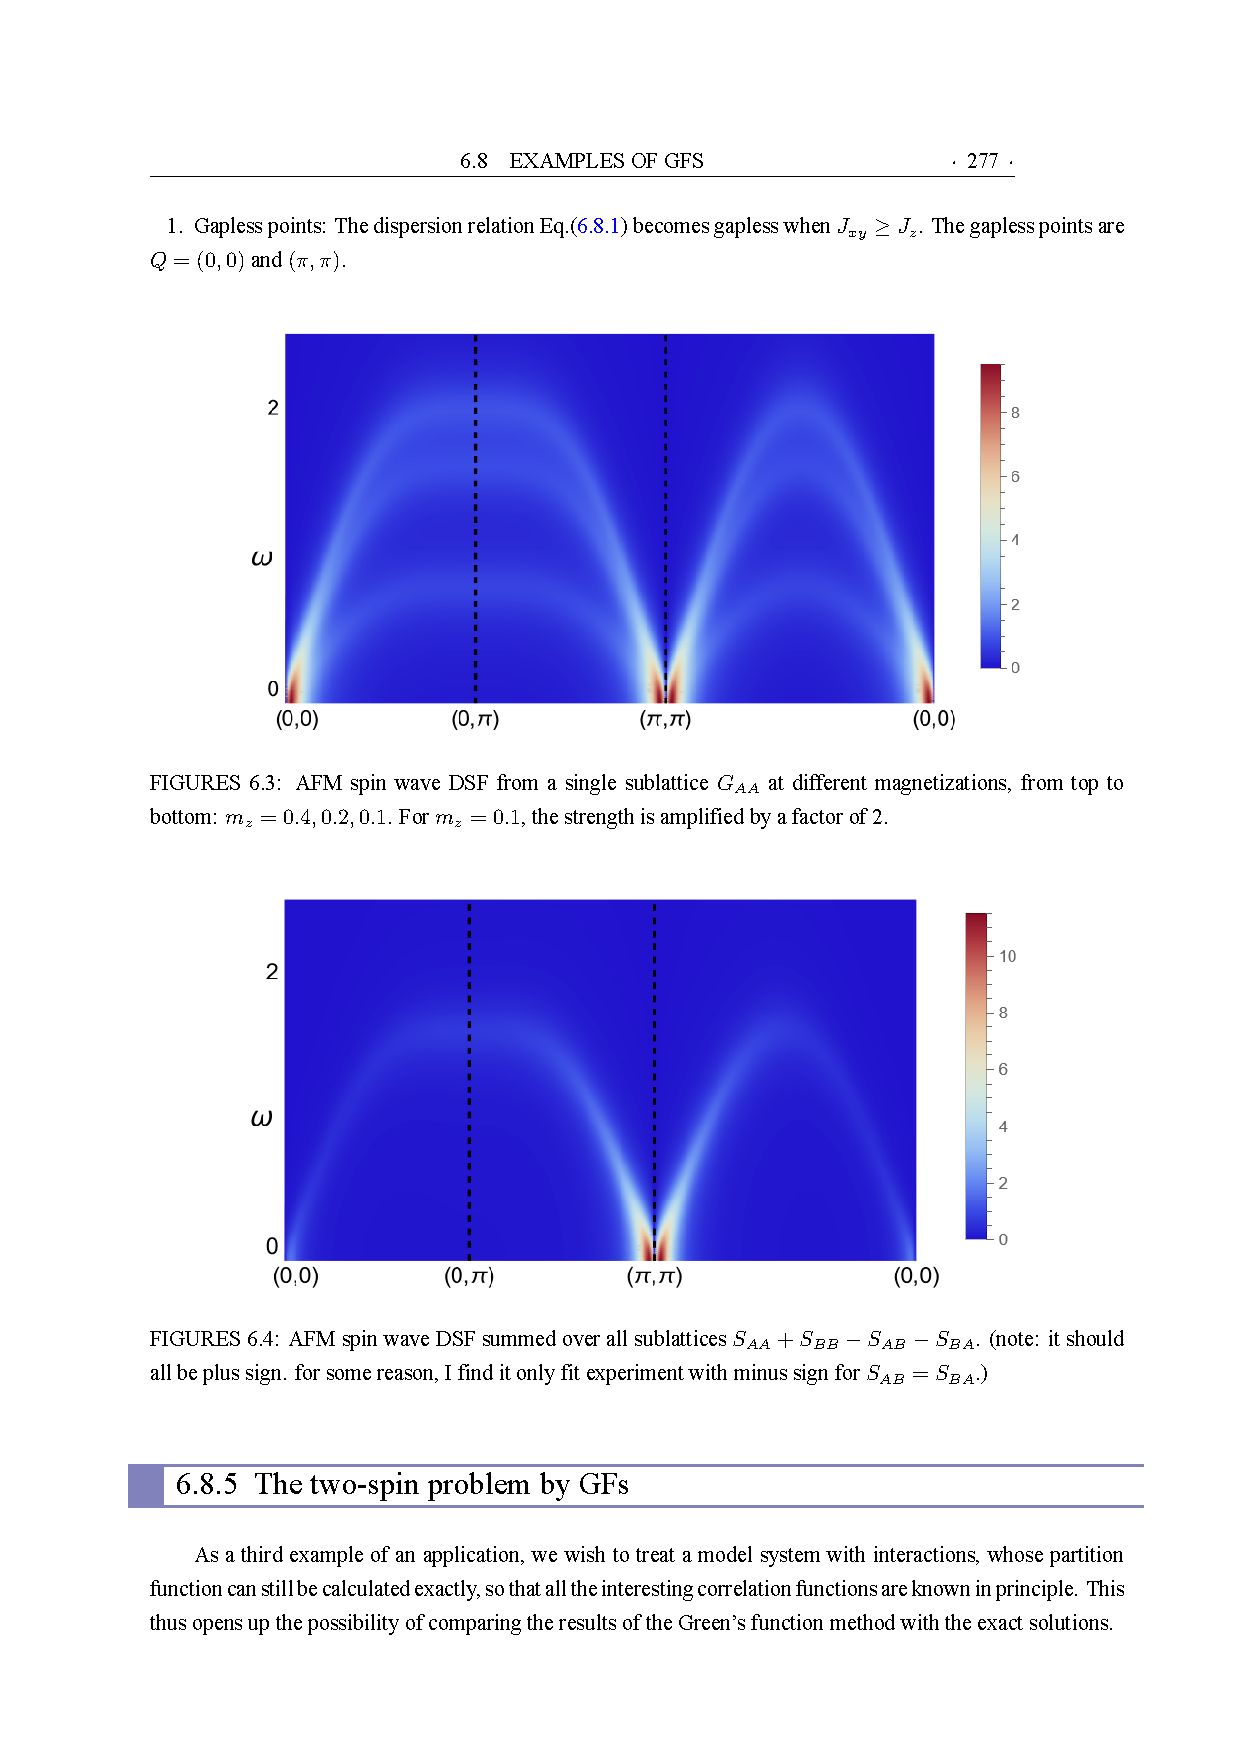
\includegraphics [width = \linewidth, page = 1] {media/GFs}
  \end{minipage}
  \hspace*\fill
  \begin{minipage}{.48\linewidth}
    \centering
    \includegraphics [width = \linewidth, page = 2] {media/GFs}
  \end{minipage}
\end{center}
Roton: liquid \ce{He}.
Roton get deeper during the salivation process.

\section{Quasi-Particle Concept}

\begin{equation}
  \iu\pdif t G_{AB} = \delta(t) \braket<[A,B]>_\xi(t = 0) + \braket<[A,H],B>
= \delta(t) \cdots + \epsilon_k G_0 + \Gamma
\end{equation}
where $\theta(t - t')AB = \theta(t' - t) BA$.
$\braket<[A,H],B>$ is the so-called vertex function $\Gamma = \sum G$, $H = H_0 + V$.
Then, we have the Dyson equation
\begin{equation}
  G_{k\sigma}(E) = G_{k\sigma}^0 + G_k(E)^0 \Sigma(k, E) G_{k\sigma}(E)
\end{equation}
and we can solve the Green function formally as
\begin{equation}
  G_{k\sigma}(E) = \frac1{E - \epsilon_k + \Sigma}, \qq{where}
  G_k^0 = \frac1{E - \epsilon_k}
\end{equation}

\subsection{Self energy}

We assume that $\Sigma$ is the self energy.
\[
  \Sigma = \Re(k, E) + \iu\Im(k, E)
\]
we consider the relation between the advanced and retard Green function
\[
  (G^\text{adv})^* = G^\text{ret}.
\]
In particular,
\begin{equation}
  G_{k\sigma}^\text{ret}(E)
= \frac {(E - \epsilon_k + R) + \iu\identity}
        {(E - \epsilon_k + R)^2 + \iu\identity^2}
\end{equation}
and the equivalent one-electron spectral density
\begin{equation}
  S_{k\sigma}(E) = -\frac1\pi \frac\identity{(E - \epsilon_k + R)^2 + I^2}
\end{equation}

\paragraph{Case A\quad $I = 0$}

Denote $I \to -0^+$. The $\delta$-function becomes
\[
  \delta(E - E_0) = \frac1\pi \lim_{x\to0} \frac x{(E - E_0)^2 + x^2}
\]
Then the equivalent one-electron spectral density becomes
\begin{equation}
  S_k(E) = \delta(E - \epsilon_k + R)
\end{equation}
To get the solution, let the $\delta$-function to be $1$
\[
  E - \epsilon_k + R = 0, \Rightarrow E_i(k)
\]
then, we have
\[
  \delta(E - \epsilon_k + R) = S(E)
= \sum \alpha_i(k) \delta(E - E_i(k)), \qq{and}
  \alpha_i(k) = \ab|1 - \pdv*{k(E)}E|^{-1}
\]
where make use of
\[
  \delta[f(x)] = \sum_i \frac1{f'(x_i)} \delta(x - x_i)
\]

\paragraph{Case B\quad $I \neq 0$}

\begin{align*}
  & \braket<S^+|S^-> \to \braket<\psi(t')|\psi(t)>
  \xlongrightarrow{t-t'\to\infty} \text{Const} \to 0;\\
  & \braket<c|c^\dagger>
\end{align*}
means $\ket|\psi> = S^-\ket|\Psi_0>$ is no longer eigenstate.
Particle will decay.
\[
  |I| \ll |\epsilon_k + R|
\]
Since
\[
  F = \epsilon_k + R
= F(E_i) + (E - E_i)\pdv FE\bigg|_{E=E_i} + \cdots
= E_i + (E - E_i)\pdv FE\bigg|_{E=E_i} + \cdots
\]
Then, the element of the density satisfies
\begin{equation}
  S^{(i)} \approxeq \alpha_i \upe^{-\iu E_i(t-t')}
\end{equation}
and we call the lifetime of quasi-particles $\upe^{-|\alpha \identity||t-t'|} \to \upe^{-|t-t'|/\tau}$, where the lifetime $\tau = 1/|\alpha I|$.
The Real part $\Re[\Sigma]$ and the imaginary part $\Im[\Sigma]$ are \emph{not independent} from each other.
\begin{align}
  \epsilon_k & \approxeq T_0 + \frac{k^2}{2m}\\
  E_i & = T_0 + \frac{k^2}{2m^*}
\end{align}
then, we have
\[
  E_i = T_0 + \frac m{m^*}(\epsilon_k - T_0),
\]
and the fraction of $m$ and $m^*$
\[
  \frac{m}{m^*} = \pdv{E_i(k)}{\epsilon_k} = 1 + \pdv R{\epsilon_k}
= 1 + \pdv R{E_i} \pdv{E_i}k
= \frac{1 - \ab(\pdv R{E_i})_{\epsilon_k}}{1 + \ab(\pdv R{\epsilon_k})_{E_i}}
\]
\input{chapter/7_.tex}

\printbibliography[title = {\refname\label{chap:bibliography}}]
\newcommand \sectionname {Lecture \#}
\appendix
\sidefoot \thepage
\fancyhead[OL, ER]{Mingyu Xia (Westlake ID: 20251202247)}
\fancyhead[EL]{\sffamily \rightmark}
\fancyhead[OR]{\fontfamily{lmr}\selectfont<<\texttt{\href{mailto:xiamingyu@westlake.edu.cn}{xiamingyu@westlake.edu.cn}}>>}
\addcontentsline{toc}{chapter}{Problem Set}
\renewcommand *\thesection{\sectionname \arabic{section}}
\newweek
\input{homework/week1.tex}
\newweek
\input{homework/week2.tex}
\newweek
\input{homework/week3.tex}
\newweek
\input{homework/week4.tex}
\newweek
\input{homework/week5.tex}
\newweek
\input{homework/week6.tex}
\newweek
\input{homework/week7.tex}
\newweek
\input{homework/week8.tex}
\newweek
% !TeX root = ../main.tex

\section{Homework \#9 [2025-11-04]}

\begin{problem}
  Calculate the Landau parameters to leading order in $\lambda_{1,2}$ for a
  Fermi liquid with the contact interactions
  \begin{enumext}
    \item $V(x - x') = \lambda_1\delta^{(3)}(x - x')$.
    \item $V(x - x') = -\lambda_2\nabla^2\delta^{(3)}(x - x')$
          (so that $V(q) = \lambda_1 q^2$ in Fourier space).
    \item Taking the results of (a) and (b) literally, sketch the regions of
          the $\lambda_1$, $\lambda_2$ phase diagram where the Fermi surface
          becomes unstable.
  \end{enumext}
\end{problem}
\begin{solution}\leavevmode
  \begin{enumext}
    \item 
  \end{enumext}
\end{solution}

\begin{problem}
  Test your understanding of Landau's mass renormalization formula by
  generalizing it to include the effect of a magnetization. Suppose we introduce
  a second vector potential into \eqref{6.86}
  \begin{equation}
    A(\theta) \underset{|\bm k|\to0}\sim \int_{k_F-k\cos\theta}^{k_F} \d q
    \frac{2\iu\pi a^2}{\omega - v_F(|\bm k + \bm q| - q)}
  = \frac{2\iu\pi a^2k\cos\theta}{\omega - v_Fk\cos\theta}.
    \tag{6.86} \label{6.86}
  \end{equation}
  that couples to the spin current, writing
  \[
    \mathcal H[\mathbf A_N, \mathbf W]
  = \sum_\sigma \int \d^3x \frac1{2m} \psi_\sigma^\dagger(x)
    [(-\iu\hbar\nabla - \mathbf A_N - \sigma\mathbf W)^2] \psi_\sigma(x)
  + \hat V
  \]
  Whereas $\mathbf A_N$ couples to the current of particles, $\mathbf W$
  couples to the ($z$ component of the) spin current.
  Assume that $V$ conserves spin current.
  \begin{enumext}
    \item By comparing the bare shift of the energies
    \[
      \delta\epsilon_{\mathbf p\sigma}^{(0)}
    = -\frac{\mathbf p}{m} \cdot (\mathbf A_N + \sigma \mathbf W)
    \]
    with the shift that result from interaction feedback,
    \[
      \delta\epsilon_{\mathbf p\sigma}
    = -\frac{\mathbf p}{m^*} \cdot \mathbf A_N
    - \sigma \frac{\mathbf p}{m_s^*} \cdot \mathbf W,
    \]
    show that there are two different mass renormalizations,
    \begin{align*}
      \frac{m}{m^*}   & = \frac1{1 + F_1^s},\\
      \frac{m}{m_s^*} & = \frac1{1 + F_1^a}.
    \end{align*}
    \item Show that, when the Fermi liquid is polarized, the masses of the
    ``up'' and ``down'' quasiparticles are now different, and given by
    \[
      \frac1{m_\sigma^*} = \frac1m\ab[\frac1{1 + F_1^s} + \frac M{1 + F_1^a}],
      \quad (\sigma = \uparrow, \downarrow)
    \]
    where the magnetization $M = n_\uparrow - n_\downarrow$ is the difference of
    ``up'' and ``down'' densities.
  \end{enumext}
\end{problem}
\begin{solution}\leavevmode
  \begin{enumext}
    \item 
  \end{enumext}
\end{solution}

\end{document}